\documentclass[12pt,onecolumn]{article}

% Page configurations
\title{GATE 2020: MECHANICAL ENGINEERING}

\usepackage[a4paper,bottom=1in,top=1in]{geometry}
\usepackage{amsmath}
\usepackage{graphicx}
\usepackage{float}
\usepackage{multicol}
\usepackage{multirow}
\setlength{\columnsep}{1cm}
\usepackage{gvv}
\graphicspath{{figs/}}

\begin{document}

\begin{center}
    \LARGE\textbf{ME: MECHANICAL ENGINEERING}\\
    \Large\textbf{SESSION - 1}
\end{center}

\noindent\large\textbf{GA - General Aptitude}\\
\normalsize\textbf{Q1 - Q5 carry one mark each.}

\begin{enumerate}
    \item He is known for his unscrupulous ways. He always sheds \underline{\hspace{2cm}} tears to deceive people.
          \begin{enumerate}
              \begin{multicols}{4}
                  \item fox's
                  \item crocodile's
                  \item crocodile
                  \item fox
              \end{multicols}
          \end{enumerate}

    \item Jofra Archer, the England fast bowler, is \underline{\hspace{2cm}} than accurate.
          \begin{enumerate}
              \begin{multicols}{4}
                  \item more fast
                  \item faster
                  \item less fast
                  \item more faster
              \end{multicols}
          \end{enumerate}

    \item Select the word that fits the analogy:\\Build : Building :: Grow : \underline{\hspace{2cm}}
          \begin{enumerate}
              \begin{multicols}{4}
                  \item Grown
                  \item Grew
                  \item Growth
                  \item Growed
              \end{multicols}
          \end{enumerate}

    \item I do not think you know the case well enough to have opinions. Having said that, I agree with your other point.\\
          What does the phrase "having said that" mean in the given text?
          \begin{enumerate}
              \begin{multicols}{4}
                  \item as opposed to what I have said
                  \item despite what I have said
                  \item in addition to what I have said
                  \item contrary to what I have said
              \end{multicols}
          \end{enumerate}

    \item Define $[x]$ as the greatest integer less than or equal to $x$, for each $x \in (-\infty, \infty)$. If $y = [x]$ then area under $y$ for $x \in [1, 4]$ is \underline{\hspace{2cm}}.
          \begin{enumerate}
              \begin{multicols}{4}
                  \item 1
                  \item 3
                  \item 4
                  \item 6
              \end{multicols}
          \end{enumerate}
\end{enumerate}
\normalsize\textbf{Q6 - Q10 carry two marks each.}

\begin{enumerate}
    \setcounter{enumi}{5}
    \item Crowd funding deals with mobilization of funds for a project from a large number of people, who would be willing to invest smaller amounts through web-based platforms in the project.\\\\Based on the above paragraph, which of the following is correct about crowd funding?
          \begin{enumerate}
              \begin{multicols}{4}
                  \item Funds raised through unwilling contributions on web-based platforms.
                  \item Funds raised through large contributions on web-based platforms.
                  \item Funds raised through coerced contributions on web-based platforms.
                  \item Funds raised through voluntary contributions on web-based platforms.
              \end{multicols}
          \end{enumerate}

    \item P, Q, R and S are to be uniquely coded using $\alpha$ and $\beta$. If P is coded as $\alpha\alpha$ and Q as $\alpha\beta$, then R and S, respectively, can be coded as \underline{\hspace{2cm}}.
          \begin{enumerate}
              \begin{multicols}{4}
                  \item $\beta\alpha$ and $\alpha\beta$
                  \item $\beta\beta$ and $\alpha\alpha$
                  \item $\alpha\beta$ and $\beta\beta$
                  \item $\beta\alpha$ and $\beta\beta$
              \end{multicols}
          \end{enumerate}

    \item The sum of first n terms in the sequence 8, 88, 888, 8888, ... is \underline{\hspace{2cm}}.
          \begin{enumerate}
              \item $\frac{81}{80}(10^n-1)+\frac{9}{8}n$
              \item $\frac{81}{80}(10^n-1)-\frac{9}{8}n$
              \item $\frac{80}{81}(10^n-1)+\frac{8}{9}n$
              \item $\frac{80}{81}(10^n-1)-\frac{8}{9}n$
          \end{enumerate}

    \item Select the graph that schematically represents BOTH $y=x^m$ and $y=x^{1/m}$ properly in the interval $0\le x \le 1$, for integer values of $m$, where $m > 1$.
          \begin{enumerate}
              \item 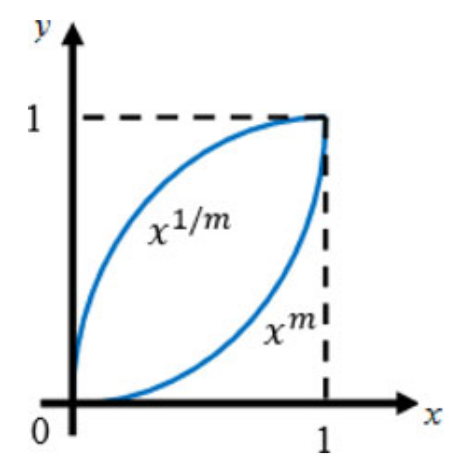
\includegraphics[scale=0.2]{o9a}
              \item 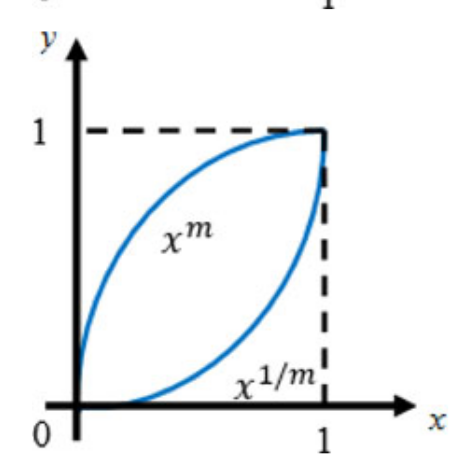
\includegraphics[scale=0.2]{o9b}
              \item 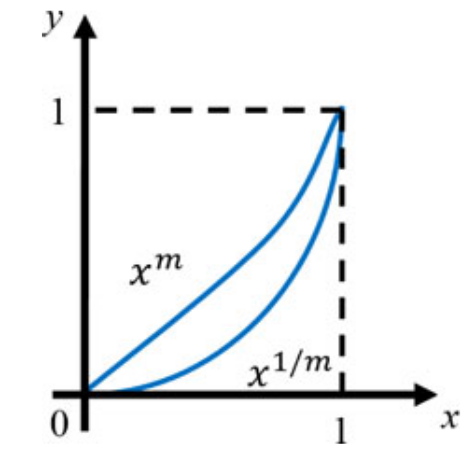
\includegraphics[scale=0.2]{o9c}
              \item 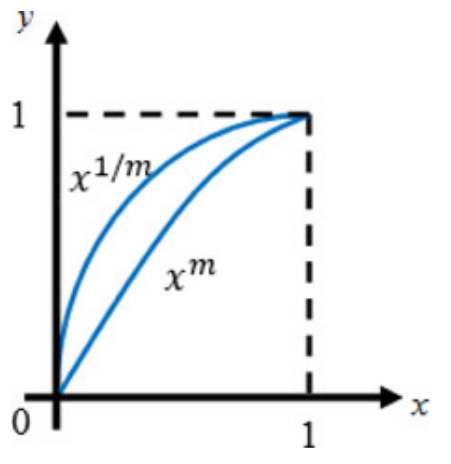
\includegraphics[scale=0.2]{o9d}
          \end{enumerate}

    \item The bar graph shows the data of the students who appeared and passed in an examination for four schools P, Q, R and S. The average of success rates (in percentage) of these four schools is \underline{\hspace{2cm}}.
          \begin{figure}[H]
              \centering
              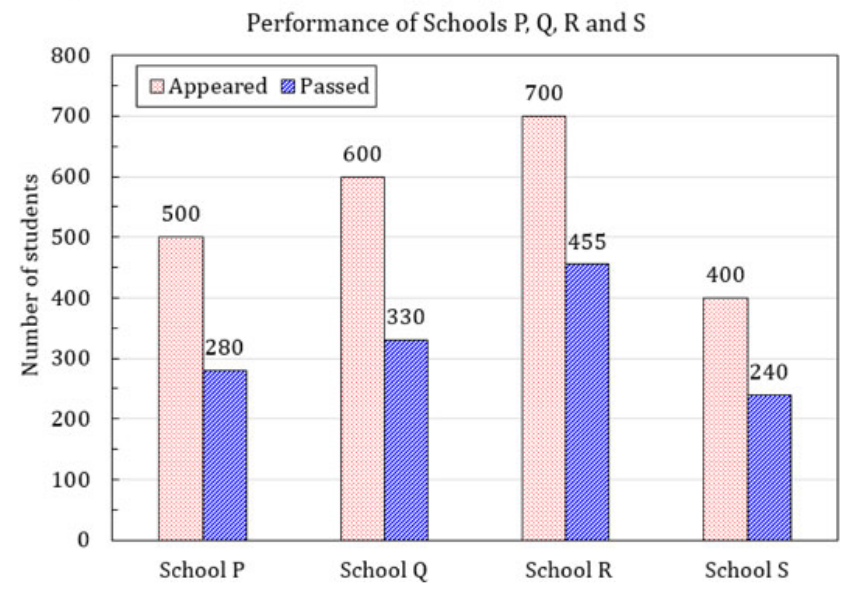
\includegraphics[scale=0.4]{q10}
              \label{fig:q10}
          \end{figure}
          \begin{enumerate}
              \item 58.5\%
              \item 58.8\%
              \item 59.0\%
              \item 59.3\%
          \end{enumerate}

\end{enumerate}

\noindent\large\textbf{ME1: Mechanical Engineering}\\
\normalsize\textbf{Q1 - Q25 carry one mark each.}
\begin{enumerate}
    \item Multiplication of real valued square matrices of same dimension is
          \begin{enumerate}
              \begin{multicols}{2}
                  \item associative
                  \item commutative
                  \item always positive definite
                  \item not always possible to compute
              \end{multicols}
          \end{enumerate}

    \item The value of
          \[
              \lim_{x\to1} \left( \frac{1-e^{-c(1-x)}}{1-xe^{-c(1-x)}} \right)
          \] is
          \begin{enumerate}
              \begin{multicols}{4}
                  \item $c$
                  \item $c+1$
                  \item $\frac{c}{c+1}$
                  \item $\frac{c+1}{c}$
              \end{multicols}
          \end{enumerate}

    \item The Laplace transformation of a function $f(t)$ is $\mathcal{L}(f)=\frac{1}{(s^2+\omega^2)}$. Then $f(t)$ is
          \begin{enumerate}
              \begin{multicols}{2}
                  \item $f(t)=\frac{1}{\omega^2}(1-\cos(\omega t))$
                  \item $f(t)=\frac{1}{\omega}\cos(\omega t)$
                  \item $f(t)=\frac{1}{\omega}\sin(\omega t)$
                  \item $f(t)=\frac{1}{\omega^2}(1-\sin(\omega t))$
              \end{multicols}
          \end{enumerate}

    \item Which of the following function $f(z)$, of the complex variable $z$, is \textbf{NOT} analytic at all the points of the complex plane?
          \begin{enumerate}
              \begin{multicols}{4}
                  \item $f(z)=z^2$
                  \item $f(z)=e^z$
                  \item $f(z)=\sin z$
                  \item $f(z)=\log z$
              \end{multicols}
          \end{enumerate}

    \item The members carrying zero force (i.e. zero-force members) in the truss shown in the figure, for any load $P>0$ with no appreciable deformation of the truss (i.e. with no appreciable change in angles between the members), are
          \begin{figure}[H]
              \centering
              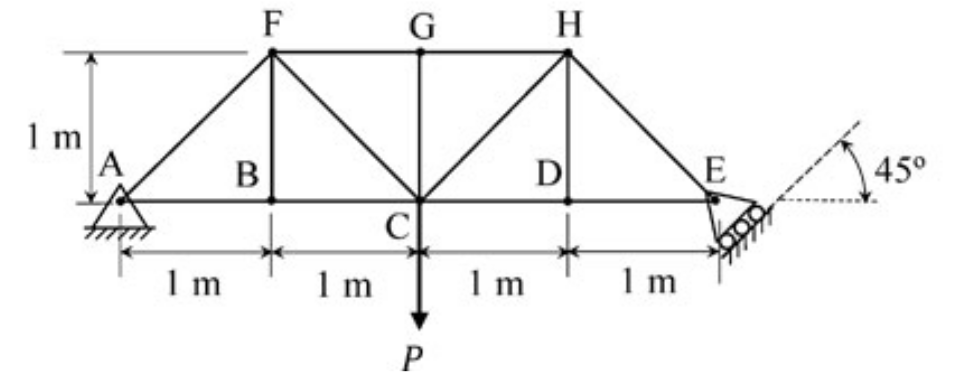
\includegraphics[scale=0.4]{q5}
              \label{fig:q5}
          \end{figure}
          \begin{enumerate}
              \begin{multicols}{2}
                  \item BF and DH only
                  \item BF, DH and GC only
                  \item BF, DH, GC, CD and DE only
                  \item BF, DH, GC, FG and GH only
              \end{multicols}
          \end{enumerate}

    \item A single-degree-of-freedom oscillator is subjected to harmonic excitation $F(t) = F_0\cos(\omega t)$ as shown in the figure.
          \begin{figure}[H]
              \centering
              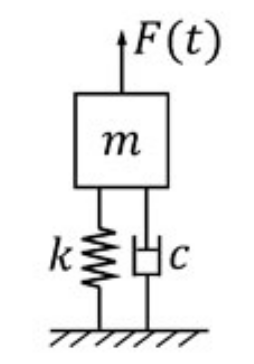
\includegraphics[scale=0.4]{q6}
              \label{fig:q6}
          \end{figure}
          The non-zero value of $\omega$, for which the amplitude of the force transmitted to the ground will be $F_0$, is
          \begin{enumerate}
              \begin{multicols}{4}
                  \item $\sqrt{\frac{k}{2m}}$
                  \item $\sqrt{\frac{k}{m}}$
                  \item $\sqrt{\frac{2k}{m}}$
                  \item $2\sqrt{\frac{k}{m}}$
              \end{multicols}
          \end{enumerate}

    \item The stress state at a point in a material under plane stress condition is equi-biaxial tension with a magnitude of 10 MPa. If one unit on the $\sigma-\tau$ plane is 1MPa, the Mohr's circle representation of the state-of-stress is given by
          \begin{enumerate}
              \item a circle with a radius equal to the principal stress and its center at the origin of the $\sigma-\tau$ plane
              \item a point on the $\sigma$ axis at a distance of 10 units from the origin
              \item a circle with a radius of 10 units on the $\sigma-\tau$ plane
              \item a point on the $\tau$ axis at a distance of 10 units from the origin
          \end{enumerate}

    \item A four bar mechanism is shown below.
          \begin{figure}[H]
              \centering
              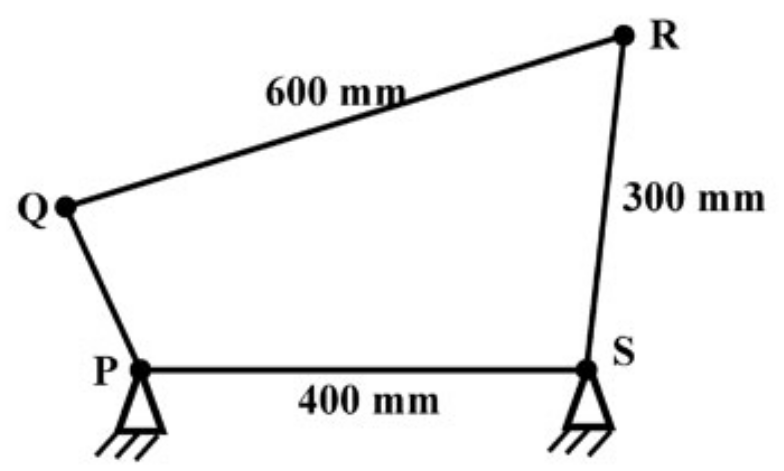
\includegraphics[scale=0.4]{q8}
              \label{fig:q8}
          \end{figure}
          For the mechanism to be a crank-rocker mechanism, the length of the link PQ can be
          \begin{enumerate}
              \begin{multicols}{4}
                  \item 80 mm
                  \item 200 mm
                  \item 300 mm
                  \item 350 mm
              \end{multicols}
          \end{enumerate}

    \item A helical gear with 20$^\circ$ pressure angle and 30$^\circ$ helix angle mounted at the mid-span of a shaft that is supported between two bearings at the ends. The nature of the stresses induced in the shaft is
          \begin{enumerate}
              \item normal stress due to bending only
              \item normal stress due to bending in one plane and axial loading; shear stress due to torsion
              \item normal stress due to bending in two planes and axial loading; shear stress due to torsion
              \item normal stress due to bending in two planes; shear stress due to torsion
          \end{enumerate}

    \item The crystal structure of $\gamma$ iron (austenite phase) is
          \begin{enumerate}
              \begin{multicols}{4}
                  \item BCC
                  \item FCC
                  \item HCP
                  \item BCT
              \end{multicols}
          \end{enumerate}

    \item Match the following.
          \begin{table}[H]
              \centering\large
              \begin{tabular}{|l|l|}
                  \hline
                  \textbf{Heat treatment process} & \textbf{Effect}  \\
                  \hline
                  P: Tempering                    & 1. Strengthening \\\hline
                  Q: Quenching                    & 2. Toughening    \\\hline
                  R: Annealing                    & 3. Hardening     \\\hline
                  S: Normalizing                  & 4. Softening     \\\hline
              \end{tabular}
              \label{tab:q11}
          \end{table}
          \begin{enumerate}
              \item P-2, Q-3, R-4, S-1
              \item P-1, Q-1, R-3, S-2
              \item P-3, Q-3, R-1, S-3
              \item P-4, Q-3, R-2, S-1
          \end{enumerate}

    \item The base of a brass bracket needs rough grinding. For this purpose, the most suitable grinding wheel grade specification is
          \begin{enumerate}
              \begin{multicols}{4}
                  \item C30Q12V
                  \item A50G8V
                  \item C90J4B
                  \item A30D12V
              \end{multicols}
          \end{enumerate}

    \item In the Critical Path Method (CPM), the cost-time slope of an activity is given by
          \begin{enumerate}
              \item $\frac{\text{Crash Cost} - \text{Normal Cost}}{\text{Crash Time}}$
              \item $\frac{\text{Normal Cost}}{\text{Crash Time} - \text{Normal Time}}$
              \item $\frac{\text{Crash Cost}}{\text{Crash Time} - \text{Normal Time}}$
              \item $\frac{\text{Crash Cost} - \text{Normal Cost}}{\text{Normal Time} - \text{Crash Time}}$
          \end{enumerate}

    \item Froude number is the ratio of
          \begin{enumerate}
              \begin{multicols}{2}
                  \item buoyancy forces to viscous forces
                  \item inertia forces to viscous forces
                  \item buoyancy forces to inertia forces
                  \item inertia forces to gravity forces
              \end{multicols}
          \end{enumerate}

    \item Match the following non-dimensional numbers with the corresponding definitions:
          \begin{table}[H]
              \centering\large
              \begin{tabular}{|c|c|c|c|}
                  \hline
                  \multicolumn{2}{|c|}{\textbf{Non-dimensional number}} & \multicolumn{2}{|c|}{\textbf{Definition}}                                                                                 \\
                  \hline
                  P                                                     & Reynolds number                           & 1 & $\frac{\text{Buoyancy force}}{\text{Viscous force}}$                      \\\hline
                  Q                                                     & Grashof number                            & 2 & $\frac{\text{Momentum diffusivity}}{\text{Thermal diffusivity}}$          \\\hline
                  R                                                     & Nusselt number                            & 3 & $\frac{\text{Inertia force}}{\text{Viscous force}}$                       \\\hline
                  S                                                     & Prandtl number                            & 4 & $\frac{\text{Convective heat transfer}}{\text{Conduction heat transfer}}$ \\\hline
              \end{tabular}
              \label{tab:q15}
          \end{table}
          \begin{enumerate}
              \item P-1, Q-3, R-2, S-4
              \item P-3, Q-1, R-2, S-4
              \item P-4, Q-3, R-1, S-2
              \item P-3, Q-1, R-4, S-2
          \end{enumerate}

    \item The velocity of an incompressible flow in a Cartesian system is represented by
          \[
              \vec{V} = 2(x^2-y^2)\hat{i} + v\hat{j} + 3\hat{k}
          \]
          Which one of the following expressions for $v$ is invalid?
          \begin{enumerate}
              \begin{multicols}{2}
                  \item $-4xz + 6xy$
                  \item $-4xy - 4xz$
                  \item $4xz - 6xy$
                  \item $4xy + 4xz$
              \end{multicols}
          \end{enumerate}

    \item For an ideal gas, the value of the Joule-Thomson coefficient is
          \begin{enumerate}
              \begin{multicols}{2}
                  \item positive
                  \item negative
                  \item zero
                  \item indeterminate
              \end{multicols}
          \end{enumerate}

    \item For an ideal gas, a constant pressure line and a constant volume line intersect at a point, in the Temperature ($T$) versus specific entropy ($s$) diagram. $C_P$ is the specific heat at constant pressure and $C_V$ is the specific heat at constant volume. The ratio of the slopes of the constant pressure and constant volume lines at the point of intersection is.
          \begin{enumerate}
              \begin{multicols}{2}
                  \item $\frac{C_P-C_V}{C_P}$
                  \item $\frac{C_P}{C_V}$
                  \item $\frac{C_P-C_V}{C_V}$
                  \item $\frac{C_V}{C_P}$
              \end{multicols}
          \end{enumerate}

    \item For three vectors $\vec{A} = 2\hat{j} - 3\hat{k}$, $\vec{B} = -2\hat{i} + \hat{k}$ and $\vec{C} = 3\hat{i} - \hat{j}$, where $\hat{i}, \hat{j}, \hat{k}$ are unit vectors along the axes of a right-handed rectangular/Cartesian coordinate system, the value of $\left(\vec{A}\cdot\left(\vec{B}\times\vec{C}\right)+6\right)$ is \underline{\hspace{2cm}}.

    \item A flywheel is attached to an engine to keep its rotational speed between 100 rad/s and 110 rad/s. If the energy fluctuation in the flywheel between these two speeds is 1.05 kJ then the moment of inertia of the flywheel is \underline{\hspace{2cm}} kg.m$^2$ (\textit{round off to 2 decimal places}).

    \item A balanced rigid disc mounted on a rigid rotor has four identical point masses, each of 10 grams, attached to four points on the 100 mm radius circle shown in the figure.
          \begin{figure}[H]
              \centering
              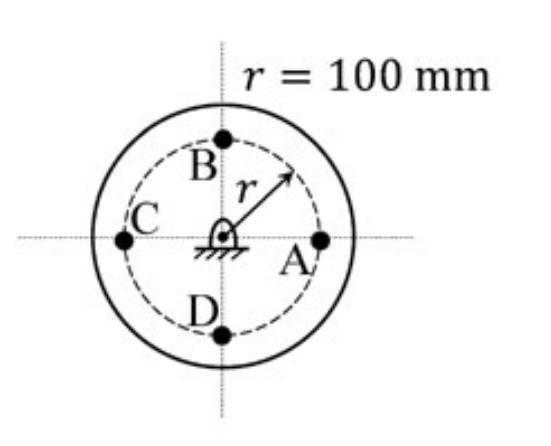
\includegraphics[scale=0.3]{q21}
              \label{fig:q21}
          \end{figure}
          The rotor is driven by a motor at uniform angular speed of 10 rad/s. If one of the masses gets detached then the magnitude of the resultant unbalance force on the rotor is \underline{\hspace{2cm}} N (\textit{round off to 2 decimal places}).

    \item A sheet metal with a stock hardness of 250 HRC has to be sheared using a punch and die having a clearance of 1 mm between them. If the stock hardness of the sheet metal increases to 400 HRC, the clearance between the punch and the die should be \underline{\hspace{2cm}} mm.

    \item A company is hiring to fill four managerial vacancies. The candidates are five men and three women. If every candidate is equally likely to be chosen then the probability that at least one woman will be selected is \underline{\hspace{2cm}} (\textit{round off to 2 decimal places}).

    \item The compressor of a gas turbine plant, operating on an ideal intercooled Brayton cycle, accomplishes an overall compression ratio of 6 in a two-stage compression process. Intercooling is used to cool the air coming out from the first stage to the inlet temperature of the first stage, before its entry to the second stage. Air enters the compressor at 300 K and 100 kPa. If the properties of gas are constant, the intercooling pressure for minimum compressor work is \underline{\hspace{2cm}} kPa (\textit{round off to 2 decimal places}).

    \item In a concentric tube counter-flow heat exchanger, hot oil enters at 102$^\circ$C and leaves at 65$^\circ$C. Cold water enters at 25$^\circ$C and leaves at 42$^\circ$C. The log mean temperature difference (LMTD) is \underline{\hspace{2cm}} $^\circ$C (\textit{round off to one decimal place}).
\end{enumerate}

\noindent\textbf{Q26 - Q55 carry two marks each.}
\begin{enumerate}
    \setcounter{enumi}{25}
    \item The evaluation of the definite integral $\int_{-1}^{1.4}x|x| \mathrm{d}x$ by using Simpson's 1/3$^\text{rd}$ (one-third) rule with step size $h=0.6$ yields
          \begin{enumerate}
              \begin{multicols}{4}
                  \item 0.914
                  \item 1.248
                  \item 0.581
                  \item 0.592
              \end{multicols}
          \end{enumerate}

    \item A vector field is defined as
          \[
              \vec{f}(x, y, z) = \frac{x}{\left[x^2+y^2+z^2\right]^{\frac{3}{2}}}\hat{i} + \frac{y}{\left[x^2+y^2+z^2\right]^{\frac{3}{2}}}\hat{j} + \frac{z}{\left[x^2+y^2+z^2\right]^{\frac{3}{2}}}\hat{k}
          \] where, $\hat{i}, \hat{j}, \hat{k}$ are unit vectors along the axes of a right-handed rectangular/Cartesian coordinate system. The surface integral $\iint \vec{f}\cdot\mathrm{d}\vec{S}$ (where $\mathrm{d}\vec{S}$ is an elemental surface area vector) evaluated over the inner and outer surfaces of a spherical shell formed by two concentric spheres with origin as the center, and internal and external radii of 1 and 2, respectively is
          \begin{enumerate}
              \begin{multicols}{4}
                  \item 0
                  \item $2\pi$
                  \item $4\pi$
                  \item $8\pi$
              \end{multicols}
          \end{enumerate}

    \item Bars of square and circular cross-section with 0.5 m length are made of material with shear strength of 20 MPa. The square bar cross-section dimension is 4 cm $\times$ 4 cm and the cylindrical bar cross-section diameter is 4 cm. The specimens are loaded as shown in the figure.
          \begin{figure}[H]
              \centering
              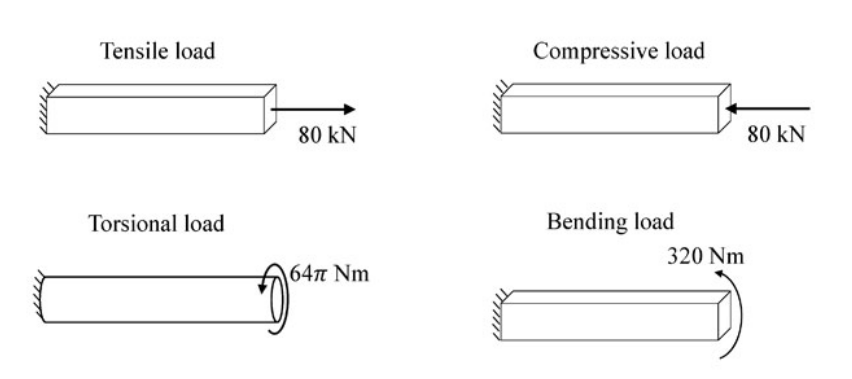
\includegraphics[scale=0.4]{q28}
              \label{fig:q28}
          \end{figure}
          Which specimen(s) will fail due to the applied load as per maximum shear stress theory?
          \begin{enumerate}
              \item Tensile and compressive load specimen
              \item Torsional load specimen
              \item Bending load specimen
              \item None of the specimen
          \end{enumerate}

    \item The 2 kg block shown in figure (top view) rests on a smooth horizontal surface and is attached to a massless elastic cord that has a stiffness 5 N/m.
          \begin{figure}[H]
              \centering
              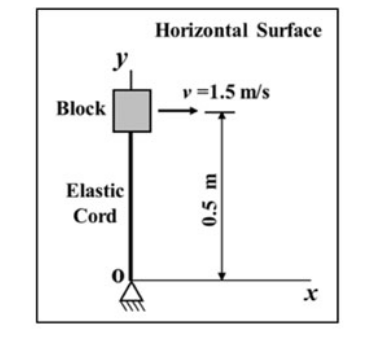
\includegraphics[scale=0.5]{q29}
              \label{fig:q29}
          \end{figure}
          The cord hinged at \textbf{O} is initially upstretched and always remains elastic. The block is given a velocity $v$ of 1.5 m/s perpendicular to the cord. The magnitude of velocity in m/s of the block at the instant the cord is stretched by 0.4 m is
          \begin{enumerate}
              \item 0.83
              \item 1.07
              \item 1.36
              \item 1.50
          \end{enumerate}

    \item The truss shown in the figure has four members of length $l$ and flexural rigidity $El$, and one member of length $l\sqrt{2}$ and flexural rigidity $4El$. The truss is loaded by a pair of forces of magnitude $P$, as shown in the figure.
          \begin{figure}[H]
              \centering
              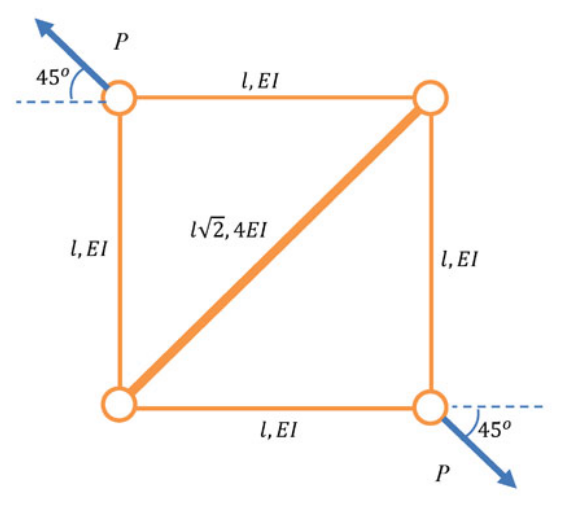
\includegraphics[scale=0.5]{q30}
              \label{fig:q30}
          \end{figure}
          The smallest value of $P$, at which any of the truss members will buckle is
          \begin{enumerate}
              \begin{multicols}{4}
                  \item $\frac{\sqrt{2}\pi^2El}{l^2}$
                  \item $\frac{\pi^2El}{l^2}$
                  \item $\frac{2\pi^2El}{l^2}$
                  \item $\frac{\pi^2El}{2l^2}$
              \end{multicols}
          \end{enumerate}

    \item A rigid mass-less rod of length $L$ is connected to a disc (pulley) of mass $m$ and radius $r=L/4$ through a friction-less revolute joint. The other end of that rod is attached to a wall through a friction-less hinge. A spring of stiffness $2k$ is attached to the rod at its mid-span. An inextensible rope passes over half the disc periphery and is securely tied to a spring of stiffness $k$ at point C as shown in the figure. There is no slip between the rope and the pulley. The system is in static equilibrium in the configuration shown in the figure and the rope is always taut.
          \begin{figure}[H]
              \centering
              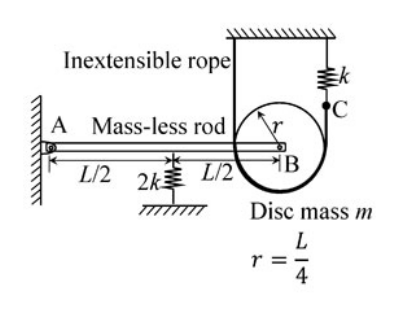
\includegraphics[scale=0.5]{q31}
              \label{fig:q31}
          \end{figure}
          Neglecting the influence of gravity, the natural frequency of the system for small amplitude vibration is
          \begin{enumerate}
              \begin{multicols}{4}
                  \item $\sqrt{\frac{3}{2}}\sqrt{\frac{k}{m}}$
                  \item $\frac{3}{\sqrt{2}}\sqrt{\frac{k}{m}}$
                  \item $\sqrt{3}\sqrt{\frac{k}{m}}$
                  \item $\sqrt{\frac{k}{m}}$
              \end{multicols}
          \end{enumerate}

    \item A strip of thickness 40 mm is to be rolled to a thickness of 20 mm using a two-high mill having rolls of diameter 200 mm. Coefficient of friction and arc length in mm, respectively are
          \begin{enumerate}
              \begin{multicols}{4}
                  \item 0.45 and 38.84
                  \item 0.39 and 38.84
                  \item 0.39 and 44.72
                  \item 0.45 and 44.72
              \end{multicols}
          \end{enumerate}

    \item For an assembly line, the production rate was 4 pieces per hour and the average processing time was 60 minutes. The WIP inventory was calculated. Now, the production rate is kept the same, and the average processing time is brought down by 30 percent. As a result of this change in the processing time, the WIP inventory
          \begin{enumerate}
              \begin{multicols}{2}
                  \item decreases by 25\%
                  \item increases by 25\%
                  \item decreases by 30\%
                  \item increases by 30\%
              \end{multicols}
          \end{enumerate}

    \item A small metal bead (radius 0.5 mm), initially at 100$^\circ$C, when placed in a stream of fluid at 20$^\circ$C, attains a temperature of 28$^\circ$C in 4.35 seconds. The density and specific heat of the metal are 8500 kg/m$^3$ and 400 J/kg.K, respectively. If the bead is considered as lumped system, the convective heat transfer coefficient (in W/m$^2$.K) between the metal bead and the fluid stream is
          \begin{enumerate}
              \begin{multicols}{4}
                  \item 283.3
                  \item 299.8
                  \item 149.9
                  \item 449.7
              \end{multicols}
          \end{enumerate}

    \item Consider two exponentially distributed random variables X and Y, both having a mean of 0.50, let Z = X+Y and r be the correlation coefficient between X and Y. If the variance of Z equals 0, then the value of $r$ is \underline{\hspace{2cm}} (\textit{round off to 2 decimal places}).
    \item An analytic function of a complex variable $z=x + iy$ $(i = \sqrt{-1})$ is defined as
          \[
              f(z) = x^2 - y^2 + i\psi(x,y),
          \]
          Where $\psi(x,y)$ is a real function. The value of the imaginary part of $f(z)$ at $z=(1+i)$ is \underline{\hspace{2cm}} (\textit{round off to 2 decimal places}).

    \item In a disc-type axial clutch, the frictional contact takes place within an annular region with outer and inner diameters 250 mm and 50 mm, respectively. An axial force $F_1$ is needed to transmit a torque by a new clutch. However, to transmit the same torque, one needs an axial force $F_2$ when the clutch wears out. If contact pressure remains uniform during operation of a new clutch while the wear is assumed to be uniform for an old clutch, and the coefficient of friction does not change, then the ratio $F_1/F_2$ is \underline{\hspace{2cm}} (\textit{round off to 2 decimal places}).

    \item A cam with a translating flat-face follower is desired to have the follower motion
          \[
              y(\theta) = 4 \left[ 2\pi\theta - \theta^2 \right],\hspace{1cm} 0 \le \theta \le 2\pi,
          \]
          Contact stress considerations dictate that the radius of curvature of the cam profile should not be less than 40 mm anywhere. The minimum permissible base circle radius is \underline{\hspace{2cm}} mm (\textit{round off to one decimal place}).

    \item A rectangular steel bar of length 500 mm, width 100 mm, and thickness 15 mm is cantilevered to a 200 mm steel channel using 4 bolts, as shown.
          \begin{figure}[H]
              \centering
              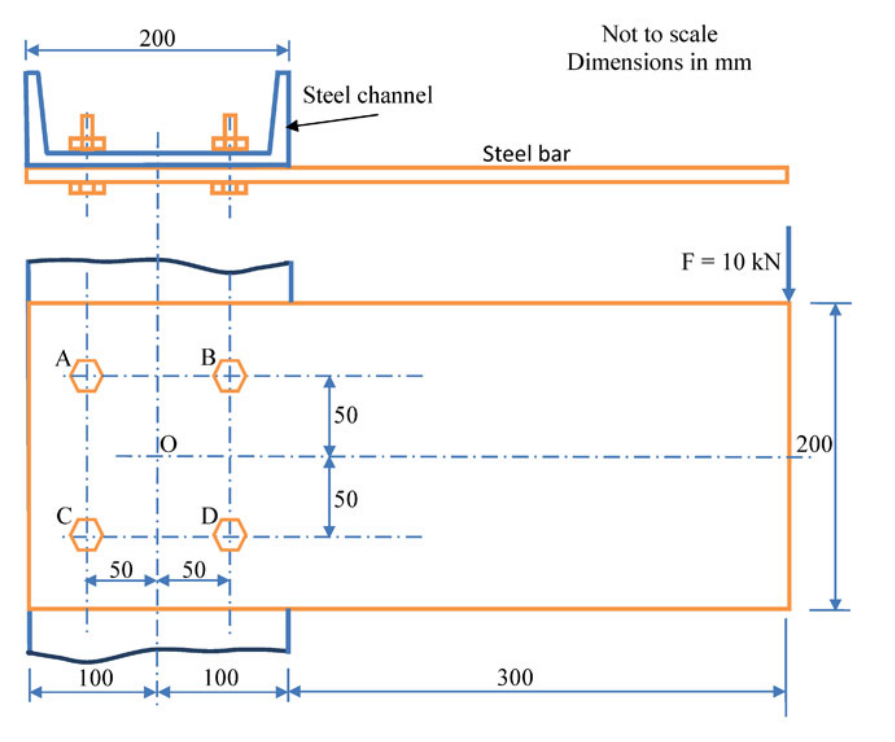
\includegraphics[scale=0.5]{q39}
              \label{fig:q39}
          \end{figure}
          For an external load of 10 kN applied at the tip of the steel bar, the resultant shear load on the bolt at B, is \underline{\hspace{2cm}} kN (\textit{round off to one decimal place}).

    \item The barrier shown between two water tanks of unit width (1 m) into the plane of the screen is modeled as a cantilever.
          \begin{figure}[H]
              \centering
              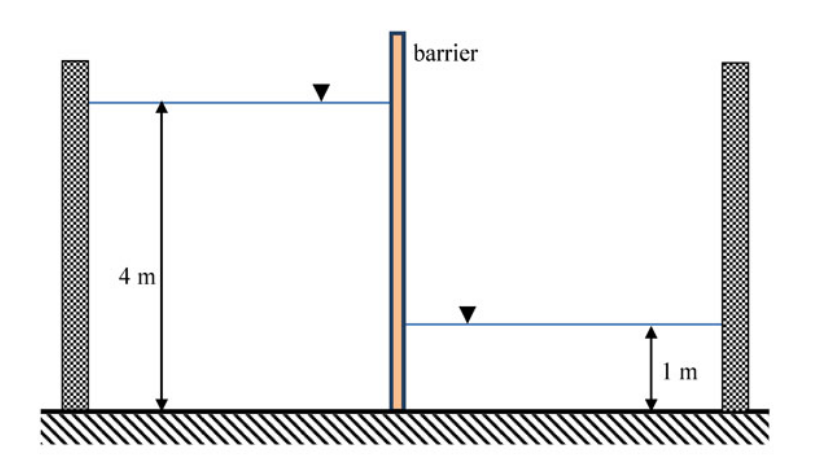
\includegraphics[scale=0.5]{q40}
              \label{fig:q40}
          \end{figure}
          Taking the density of water as 1000 kg/m$^3$ and acceleration due to gravity as 10 m/s$^2$, the maximum absolute bending moment developed in the cantilever is \underline{\hspace{2cm}} kN.m (\textit{round off to the nearest integer}).

    \item The magnitude of reaction force at joint C of the hinge-beam shown in the figure is \underline{\hspace{2cm}} kN (\textit{round off to two decimal places}).
          \begin{figure}[H]
              \centering
              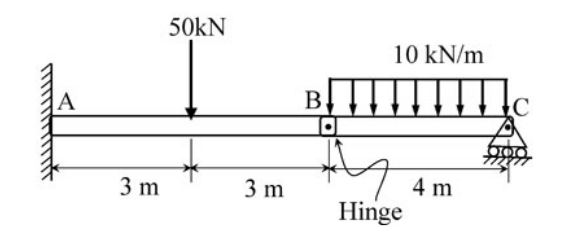
\includegraphics[scale=0.5]{q41}
              \label{fig:q41}
          \end{figure}

    \item A slot of 25 mm $\times$ 25 mm is to be milled in a workpiece of 300 mm length using a side and face milling cutter of diameter 100 mm, width 25 mm and having 20 teeth.\\\\
          For a depth of cut 5 mm, feed per tooth 0.1 mm, cutting speed 35 m/min and approach and over travel distance of 5 mm each, the time required for milling the slot is \underline{\hspace{2cm}} minutes (\textit{round off to one decimal place}).

    \item The following data applies to basic shaft system:\\
          tolerance for hole = 0.002 mm,\\
          tolerance for shaft = 0.001 mm,\\
          allowance = 0.003 mm,\\
          basic size = 50 mm.\\
          The maximum hole size is \underline{\hspace{2cm}} mm (\textit{round off to 3 decimal places}).

    \item A steel part with surface area of 125 cm$^2$ is to be chrome coated through an electroplating process using chromium acid sulphate as an electrolyte. An increasing current is applied to the part according to the following current time relation:
          \[ I = 12 + 0.2t \] where, $I = \text{current}(A)$ and $t = \text{time}(minutes)$. The part is submerged in the plating solution for a duration of 20 minutes for plating purpose. Assuming the cathode efficiency of chromium to be 15\% and the plating constant of chromium acid sulphate to be $2.50\times10^{-2} \text{mm}^3/A\cdot s$, the resulting coating thickness on the part surface is \underline{\hspace{2cm}} $\mu$m (\textit{round off to one decimal place}).

    \item In a turning process using orthogonal tool geometry, a chip length of 100 mm is obtained for an uncut chip length of 250 mm.\\\\
          The cutting conditions are: cutting speed = 30 m/min, rake angle = 20$^\circ$.\\\\
          The shear plane angle is \underline{\hspace{2cm}} degrees (\textit{round off to one decimal place}).

    \item The thickness of a steel plate with material strength coefficient of 210 MPa, has to be reduced from 20 mm to 15 mm in a single pass in a two-high rolling mill with a roll radius of 450 mm and rolling velocity of 28 m/min. If the plate has a width of 200 mm and its strain hardening exponent, n is 0.25, the rolling force required for the operation is \underline{\hspace{2cm}} kN (\textit{round off to 2 decimal places}).\\\\
          Note: \textit{Average Flow Stress = Material Strength Coefficient $\times\frac{(\text{True Strain})^n}{(1+n)}$}

    \item Two business owners Shveta and Ashok run their business in two different states. Each of them, independent of the other, produces two products A and B, sells them at Rs. 2,000 per kg and Rs. 3,000 per kg, respectively and uses Linear Programming to determine the optimal quantity of A and B to maximize their respective daily revenue. Their constraints are as follows: i) for each business owner, the production process is such that the daily production of A has to be at least as much as B, and the upper limit for production of B is 10 kg per day, and ii) the respective state regulations restrict Shveta's production of A to less than 20 kg per day, and Ashok's production of A to less than 15 kg per day. The demand of both A and B in both the states is very high and everything produced is sold.\\\\
          The absolute value of the difference in daily (optimal) revenue of Shveta and Ashok (in Rs.) is \underline{\hspace{2cm}} (\textit{round off to 2 decimal places}).

    \item \textbf{Consider two cases as below.}\\\\
          \textbf{Case 1:} A company buys 1000 pieces per year of a certain part from vendor `X'. The changeover time is 2 hours and the prices is Rs. 10 per piece. The holding cost rate per part is 10\% per year.\\\\
          \textbf{Case 2:} For the same part, another vendor `Y' offers a design where the changeover time is 6 minutes, with a prices of Rs. 5 per piece, and a holding cost rate per part of 100\% per year. The order size is 800 pieces per year from `X' and 200 pieces per year from `Y'.\\\\
          Assume the cost of downtime as Rs. 200 per hour. The percentage reduction in the annual cost for Case 2, as compared to Case 1 is \underline{\hspace{2cm}} (\textit{round off to 2 decimal places}).

    \item Consider steady, viscous, fully developed flow of a fluid through a circular pipe of internal diameter $D$. We know that the velocity profile forms a paraboloid about the pipe centre line, given by: $V=-C\left(r^2-\frac{D^2}{4}\right)$ m/s, where $C$ is a constant. The rate of kinetic energy (in J/s) at the control surface A-B, as shown in the figure, is proportional to D$^n$. The value of n is \underline{\hspace{2cm}}.
          \begin{figure}[H]
              \centering
              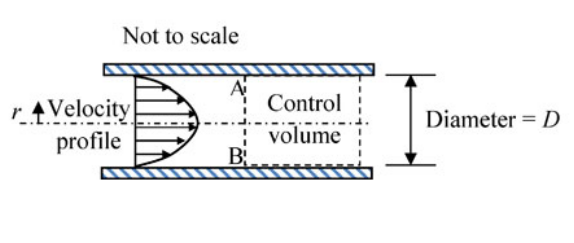
\includegraphics[scale=0.5]{q49}
              \label{fig:q49}
          \end{figure}

    \item Air discharges steadily through a horizontal nozzle and impinges on a stationary vertical plate as shown in figure.
          \begin{figure}[H]
              \centering
              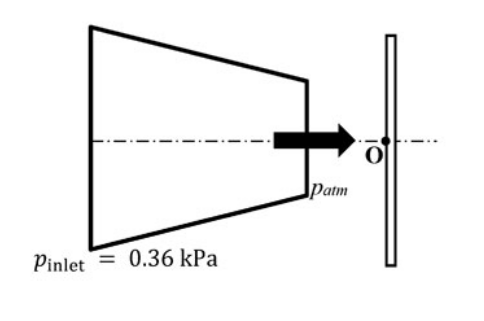
\includegraphics[scale=0.5]{q50}
              \label{fig:q50}
          \end{figure}
          The inlet and outlet areas of the nozzle are $0.1~\text{m}^2$ and $0.02~\text{m}^2$, respectively. Take air density as constant and equal to $1.2~\text{kg/m}^3$. If the inlet gauge pressure of air is $0.36~\text{kPa}$, the gauge pressure at point \textbf{O} on the plate is \underline{\hspace{2cm}} kPa (\textit{round off to two decimal places}).

    \item Air (ideal gas) enters a perfectly insulated compressor at a temperature of 310 K. The pressure ratio of the compressor is 6. Specific heat at constant pressure for air is 1005 J/kg.K and ratio of specific heats at constant pressure and constant volume is 1.4. Assume that specific heats of air are constant. If the isentropic efficiency of the compressor is 85 percent, the difference in enthalpies of air between the exit and the inlet of the compressor is \underline{\hspace{2cm}} kJ/kg (round off to nearest integer).

    \item One kg of air, initially at a temperature of 127$^\circ$C, expands reversibly at a constant pressure until the volume is doubled. If the gas constant of air is 287 J/kg.K, the magnitude of work transfer is \underline{\hspace{2cm}} kJ (\textit{round off to 2 decimal places}).

    \item For an ideal Rankine cycle operating between pressures of 30 bar and 0.04 bar, the work output from the turbine is 903 kJ/kg and the work input to the feed pump is 3 kJ/kg. The specific steam consumption is \underline{\hspace{2cm}} kg/kW.h (\textit{round off to 2 decimal places}).
    \item For a Kaplan (axial flow) turbine, the outlet blade velocity diagram at a section is shown in figure.
          \begin{figure}[H]
              \centering
              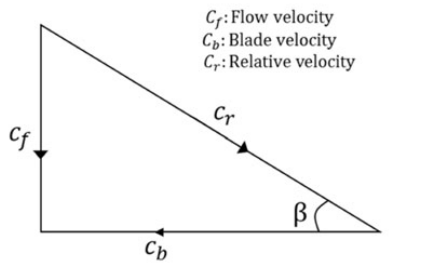
\includegraphics[scale=0.5]{q55}
              \label{fig:q55}
          \end{figure}
          The diameter at this section is 3 m. The hub and tip diameters of the blade are 2 m and 4 m, respectively. The water volume flow rate is 100 m$^3$/s. The rotational speed of the turbine is 300 rpm. The blade outlet angle $\beta$ is \underline{\hspace{2cm}} degrees (\textit{round off to one decimal place}).

    \item The indicated power developed by an engine with compression ratio of 8, is calculated using an air-standard Otto cycle (constant properties). The rate of heat addition is 10 kW. The ratio of specific heats at constant pressure and constant volume is 1.4. The mechanical efficiency of the engine is 80 percent.

          The brake power output of the engine is \underline{\hspace{2cm}} kW (\textit{round off to one decimal place}).
\end{enumerate}

\pagebreak
\begin{center}
    \Large\textbf{SESSION - 2}\\
\end{center}
\noindent\large\textbf{GA - General Aptitude}\\
\normalsize\textbf{Q1 - Q5 carry one mark each.}
\begin{enumerate}
    \item While I agree \underline{\hspace{2cm}} his proposal this time, I do not often agree \underline{\hspace{2cm}} him.
          \begin{enumerate}
              \begin{multicols}{4}
                  \item to, with
                  \item with, to
                  \item with, with
                  \item to, to
              \end{multicols}
          \end{enumerate}

    \item The recent measures to improve the output would \underline{\hspace{2cm}} the level of production to our satisfaction.
          \begin{enumerate}
              \begin{multicols}{4}
                  \item increase
                  \item decrease
                  \item speed
                  \item equalise
              \end{multicols}
          \end{enumerate}

    \item Select the word that fits the analogy:\\
          White: Whitening :: Light: \underline{\hspace{2cm}}
          \begin{enumerate}
              \begin{multicols}{4}
                  \item Lightning
                  \item Lightening
                  \item Lighting
                  \item Enlightening
              \end{multicols}
          \end{enumerate}

    \item In one of the greatest innings ever seen in 142 years of Test history, Ben Stokes upped the tempo in a five-and-a-half hour long stay of 219 balls including 11 fours and 8 sixes that saw him finish on a 135 not out as England squared the five-match series.\\
          Based on their connotations in the given passage, which one of the following meanings DOES NOT match?
          \begin{enumerate}
              \begin{multicols}{2}
                  \item upped = increased
                  \item squared = lost
                  \item tempo = enthusiasm
                  \item saw = resulted in
              \end{multicols}
          \end{enumerate}

    \item There are five levels \{P, Q, R, S, T\} in a linear supply chain before a product reaches customers, as shown in the figure.\\
          \begin{figure}[H]
              \centering
              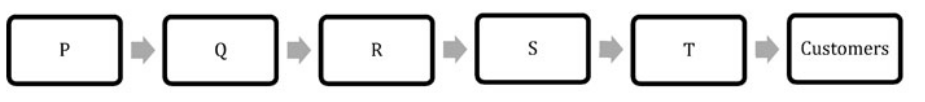
\includegraphics[scale=0.4]{q5s2}
              \label{fig:q5s2}
          \end{figure}
          At each of the five levels, the price of the product is increased by 25\%. If the product is produced at level P at the cost of Rs. 120 per unit, what is the price paid (in rupees) by the customers?
          \begin{enumerate}
              \begin{multicols}{4}
                  \item 187.50
                  \item 234.38
                  \item 292.96
                  \item 366.21
              \end{multicols}
          \end{enumerate}
\end{enumerate}
\normalsize\textbf{Q6 - Q10 carry two marks each.}
\begin{enumerate}
    \setcounter{enumi}{5}
    \item Climate change and resilience deal with two aspects – reduction of sources of non-renewable energy resources and reducing vulnerability of climate change aspects. The terms `mitigation' and `adaptation' are used to refer to these aspects, respectively.\\Which of the following assertions is best supported by this information?
          \begin{enumerate}
              \item Mitigation deals with consequences of climate change.
              \item Adaptation deals with causes of climate change.
              \item Mitigation deals with actions taken to reduce the use of fossil fuels.
              \item Adaptation deals with actions taken to combat greenhouse gas emissions.
          \end{enumerate}

    \item Find the missing element in the following figure.
          \begin{figure}[H]
              \centering
              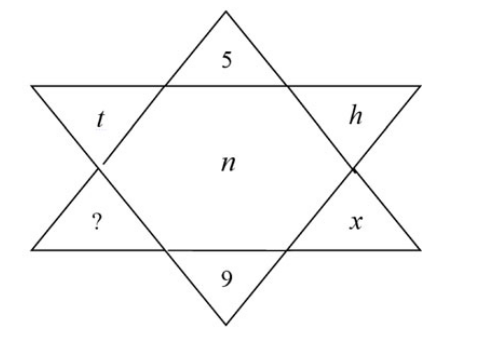
\includegraphics[scale=0.4]{q7s2}
              \label{fig:q7s2}
          \end{figure}
          \begin{enumerate}
              \begin{multicols}{4}
                  \item d
                  \item e
                  \item w
                  \item y
              \end{multicols}
          \end{enumerate}

    \item It was estimated that 52 men can complete a strip in a newly constructed highway connecting cities P and Q in 10 days. Due to an emergency, 12 men were sent to another project. How many number of days, more than the original estimate, will be required to complete the strip?
          \begin{enumerate}
              \begin{multicols}{4}
                  \item 3 days
                  \item 5 days
                  \item 10 days
                  \item 13 days
              \end{multicols}
          \end{enumerate}

    \item An engineer measures THREE quantities X, Y and Z in an experiment. She finds that they follow a relationship that is represented in the figure below: (the product of X and Y linearly varies with Z)
          \begin{center}
              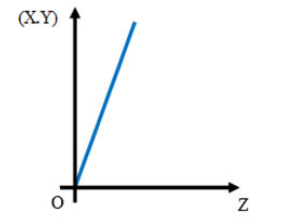
\includegraphics[scale=0.5]{q9s2}
          \end{center}
          Then, which of the following statements is FALSE?
          \begin{enumerate}
              \item For fixed Z; X is proportional to Y
              \item For fixed Y; X is proportional to Z
              \item For fixed X; Z is proportional to Y
              \item XY/Z is constant
          \end{enumerate}

    \item The two pie-charts given below show the data of total students and only girls registered in different streams in a university. If the total number of students registered in the university is 5000, and the total number of the registered girls is 1500; then, the ratio of boys enrolled in Arts to the girls enrolled in Management is \underline{\hspace{2cm}}.
          \begin{center}
              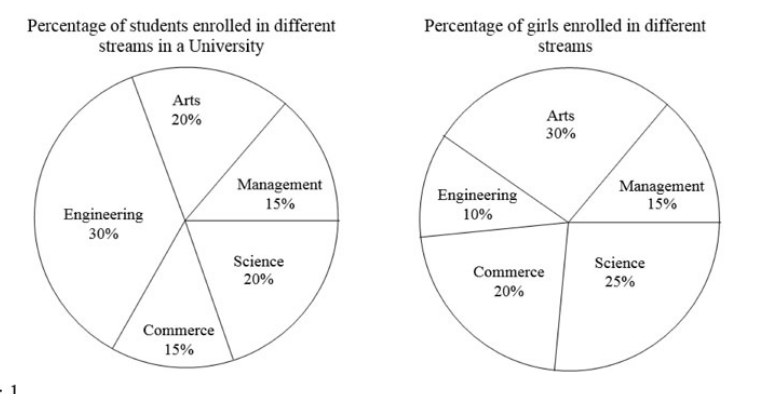
\includegraphics[scale=0.5]{q10s2}
          \end{center}
          \begin{enumerate}
              \item 2 : 1
              \item 9 : 22
              \item 11 : 9
              \item 22 : 9
          \end{enumerate}
\end{enumerate}
\noindent\large\textbf{ME2: Mechanical Engineering}\\
\normalsize\textbf{Q1 - Q25 carry one mark each.}
\begin{enumerate}
    \item The sum of two normally distributed random variables X and Y is
          \begin{enumerate}
              \item always normally distributed
              \item normally distributed, only if X and Y are independent
              \item normally distributed, only if X and Y have the same standard deviation
              \item normally distributed, only if X and Y have the same mean
          \end{enumerate}

    \item A matrix $P$ is decomposed into its symmetric part $S$ and skew symmetric part $V$. If
          \[ S = \myvec{-4 & 4 & 2 \\ 4 & 3 & 7/2 \\ 2 & 7/2 & 2}, V = \myvec{0 & -2 & 3 \\ 2 & 0 & 7/2 \\ -3 & -7/2 & 0}, \]
          then matrix $P$ is
          \begin{enumerate}
              \item $\myvec{-4 & 6 & -1 \\ 2 & 3 & 0 \\ 5 & 7 & 2}$
              \item $\myvec{-4 & 2 & 5 \\ 6 & 3 & 7 \\ -1 & 0 & 2}$
              \item $\myvec{4 & -6 & 1 \\ -2 & -3 & 0 \\ -5 & -7 & -2}$
              \item $\myvec{-2 & 9/2 & -1 \\ -1 & 81/4 & 11 \\ -2 & 45/2 & 73/4}$
          \end{enumerate}

    \item Let $I = \int_{x=0}^{1}\int_{y=0}^{x^2}xy^2~dy~dx$. Then, $I$ may also be expressed as
          \begin{enumerate}
              \item $I = \int_{y=0}^{1}\int_{x=0}^{\sqrt{y}}xy^2~dx~dy$
              \item $I = \int_{y=0}^{1}\int_{x=\sqrt{y}}^{1}yx^2~dx~dy$
              \item $I = \int_{y=0}^{1}\int_{x=\sqrt{y}}^{1}xy^2~dx~dy$
              \item $I = \int_{y=0}^{1}\int_{x=0}^{\sqrt{y}}yx^2~dx~dy$
          \end{enumerate}

    \item The solution of
          \[ \frac{d^2 y}{dt^2} - y = 1, \]
          which additionally satisfies $y\big|_{t=0} = \frac{dy}{dt}\big|_{t=0} = 0$, in the Laplace $s$-domain is
          \begin{enumerate}
              \begin{multicols}{4}
                  \item $\frac{1}{s(s+1)(s-1)}$
                  \item $\frac{1}{s(s+1)}$
                  \item $\frac{1}{s(s-1)}$
                  \item $\frac{1}{s-1}$
              \end{multicols}
          \end{enumerate}

    \item An attempt is made to pull a roller of weight $W$ over a curb (step) by applying a horizontal force $F$ as shown in the figure.
          \begin{figure}[H]
              \centering
              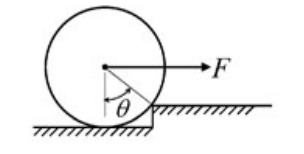
\includegraphics[scale=0.4]{q5s2mech}
              \label{fig:q5s2mech}
          \end{figure}
          The coefficient of static friction between the roller and the ground (including the edge of the step) is $\mu$. Identify the correct free body diagram (FBD) of the roller when the roller is just about to climb over the step.
          \begin{enumerate}
              \item 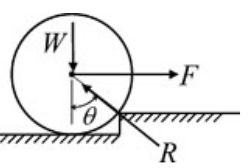
\includegraphics[scale=0.4]{o5a}
              \item 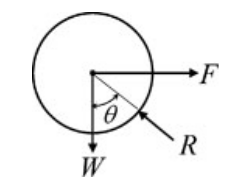
\includegraphics[scale=0.4]{o5b}
              \item 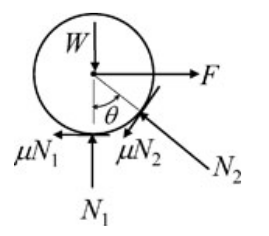
\includegraphics[scale=0.4]{o5c}
              \item 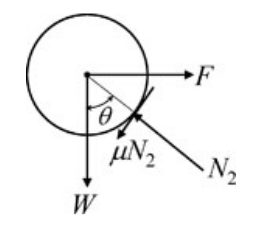
\includegraphics[scale=0.4]{o5d}
          \end{enumerate}

    \item A circular disk of radius $r$ is confined to roll without slipping at P and Q as shown in the figure.
          \begin{figure}[H]
              \centering
              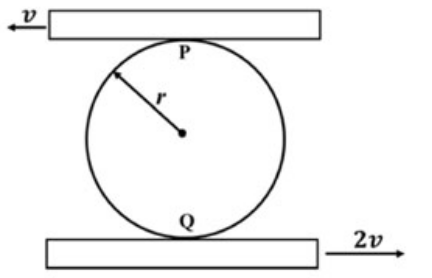
\includegraphics[scale=0.4]{q6s2}
              \label{fig:q6s2}
          \end{figure}
          If the plates have velocities shown, the magnitude of the angular velocity of the disk is
          \begin{enumerate}
              \begin{multicols}{4}
                  \item $\frac{v}{r}$
                  \item $\frac{v}{2r}$
                  \item $\frac{2v}{3r}$
                  \item $\frac{3v}{2r}$
              \end{multicols}
          \end{enumerate}

    \item The equation of motion of a spring-mass-damper system is given by
          \[ \frac{d^2x}{dt^2} + 3\frac{dx}{dt} + 9x = 10\sin(5t) \]
          The damping factor for the system is
          \begin{enumerate}
              \begin{multicols}{4}
                  \item 0.25
                  \item 0.5
                  \item 2
                  \item 3
              \end{multicols}
          \end{enumerate}

    \item The number of qualitatively distinct kinematic inversions possible for a Grashof chain with four revolute pairs is
          \begin{enumerate}
              \begin{multicols}{4}
                  \item 1
                  \item 2
                  \item 3
                  \item 4
              \end{multicols}
          \end{enumerate}

    \item The process, that uses a tapered horn to amplify and focus the mechanical energy for machining of glass, is
          \begin{enumerate}
              \item electrochemical machining
              \item electrical discharge machining
              \item ultrasonic machining
              \item abrasive jet machining
          \end{enumerate}

    \item Two plates, each of 6 mm thickness, are to be butt-welded. Consider the following processes and select the correct sequence in increasing order of size of the heat affected zone.\\\\
          \begin{enumerate}[label=\arabic*.]
              \item Arc welding
              \item MIG welding
              \item Laser beam welding
              \item Submerged arc welding
          \end{enumerate}
          \begin{enumerate}
              \item 1-4-2-3
              \item 3-4-2-1
              \item 4-3-2-1
              \item 3-2-4-1
          \end{enumerate}
    \item Which one of the following statements about a phase diagram is \textbf{INCORRECT}?
          \begin{enumerate}
              \item It indicates the temperature at which different phases start to melt
              \item Relative amount of different phases can be found under given equilibrium conditions
              \item It gives information on transformation rates
              \item Solid solubility limits are depicted by it
          \end{enumerate}

    \item The figure below shows a symbolic representation of the surface texture in a perpendicular lay orientation with indicative values (I through VI) marking the various specifications whose definitions are listed below.

          P: Maximum Waviness Height (mm); Q: Maximum Roughness Height (mm);\\
          R: Minimum Roughness Height (mm); S: Maximum Waviness Width (mm);\\
          T: Maximum Roughness Width (mm); U: Roughness Width Cutoff (mm).

          \begin{figure}[H]
              \centering
              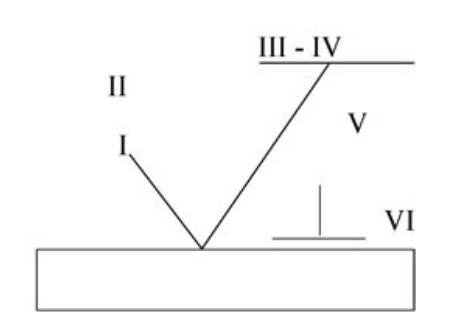
\includegraphics[scale=0.4]{q12s2}
              \label{fig:q12s2}
          \end{figure}

          The correct match between the specifications and the symbols (I to VI) is
          \begin{enumerate}
              \item I-R, II-Q, III-P, IV-S, V-U, VI-T
              \item I-R, II-P, III-U, IV-S, V-T, VI-Q
              \item I-U, II-S, III-Q, IV-T, V-R, VI-P
              \item I-Q, II-U, III-R, IV-T, V-S, VI-P
          \end{enumerate}

    \item In Materials Requirement Planning, if the inventory holding cost is very high and the setup cost is zero, which one of the following lot sizing approaches should be used?
          \begin{enumerate}
              \item Economic Order Quantity
              \item Lot-for-Lot
              \item Base Stock Level
              \item Fixed Period Quantity, for 2 periods
          \end{enumerate}

    \item Which of the following conditions is used to determine the stable equilibrium of all partially submerged floating bodies?
          \begin{enumerate}
              \item Centre of buoyancy must be above the centre of gravity
              \item Centre of buoyancy must be below the centre of gravity
              \item Metacentre must be at a higher level than the centre of gravity
              \item Metacentre must be at a lower level than the centre of gravity
          \end{enumerate}

    \item In the space above the mercury column in a barometer tube, the gauge pressure of the vapour is
          \begin{enumerate}
              \item positive, but more than one atmosphere
              \item negative
              \item zero
              \item positive, but less than one atmosphere
          \end{enumerate}

    \item A closed vessel contains pure water, in thermal equilibrium with its vapour at $25^\circ$C (Stage \#1), as shown.
          \begin{figure}[H]
              \centering
              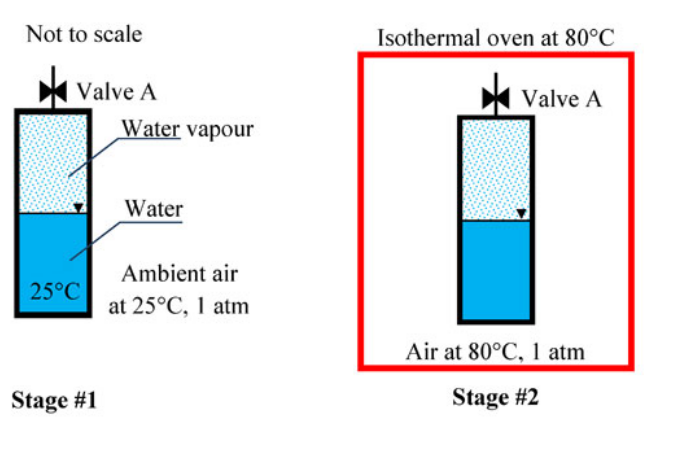
\includegraphics[scale=0.5]{q16s2}
              \label{fig:q16s2}
          \end{figure}
          The vessel in this stage is then kept inside an isothermal oven which is having an atmosphere of hot air maintained at $80^\circ$C. The vessel exchanges heat with the oven atmosphere and attains a new thermal equilibrium (Stage \#2). If the Valve A is now opened inside the oven, what will happen immediately after opening the valve?
          \begin{enumerate}
              \item Water vapor inside the vessel will come out of the Valve A
              \item Hot air will go inside the vessel through Valve A
              \item Nothing will happen -- the vessel will continue to remain in equilibrium
              \item All the vapor inside the vessel will immediately condense
          \end{enumerate}

    \item For an air-standard Diesel cycle,
          \begin{enumerate}
              \item heat addition is at constant volume and heat rejection is at constant pressure
              \item heat addition is at constant pressure and heat rejection is at constant pressure
              \item heat addition is at constant pressure and heat rejection is at constant volume
              \item heat addition is at constant volume and heat rejection is at constant volume
          \end{enumerate}

    \item The values of enthalpies at the stator inlet and rotor outlet of a hydraulic turbomachine stage are $h_1$ and $h_3$ respectively. The enthalpy at the stator outlet (or, rotor inlet) is $h_2$. The condition $(h_2 - h_1) = (h_3 - h_2)$ indicates that the degree of reaction of this stage is
          \begin{enumerate}
              \begin{multicols}{4}
                  \item zero
                  \item 50\%
                  \item 75\%
                  \item 100\%
              \end{multicols}
          \end{enumerate}

    \item Let $\mathbf{I}$ be a 100 dimensional identity matrix and $\mathbf{E}$ be the set of its distinct (no value appears more than once in $\mathbf{E}$) real eigenvalues. The number of elements in $\mathbf{E}$ is \underline{\hspace{2cm}}.

    \item A beam of negligible mass is hinged at support P and has a roller support Q as shown in the figure.
          \begin{figure}[H]
              \centering
              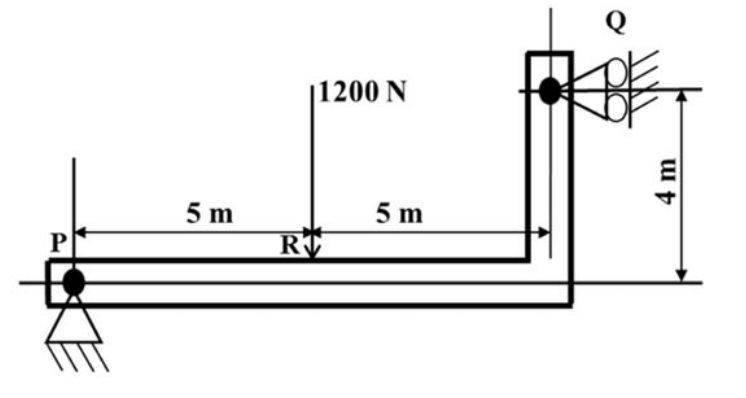
\includegraphics[scale=0.5]{q20s2}
              \label{fig:q20s2}
          \end{figure}
          A point load of 1200 N is applied at point R. The magnitude of the reaction force at support Q is \underline{\hspace{2cm}} N.

    \item A machine member is subjected to fluctuating stress $\sigma = \sigma_0 \cos(8\pi t)$. The endurance limit of the material is 350 MPa. If the factor of safety used in the design is 3.5 then the maximum allowable value of $\sigma_0$ is \underline{\hspace{2cm}} MPa (\textit{round off to 2 decimal places}).

    \item A bolt head has to be made at the end of a rod of diameter $d = 12$ mm by localized forging (upsetting) operation. The length of the unsupported portion of the rod is 40 mm. To avoid buckling of the rod, a closed forging operation has to be performed with a maximum die diameter of \underline{\hspace{2cm}} mm.

    \item Consider the following network of activities, with each activity named $\mathbf{A}$-$\mathbf{L}$, illustrated in the nodes of the network.

          \begin{figure}[H]
              \centering
              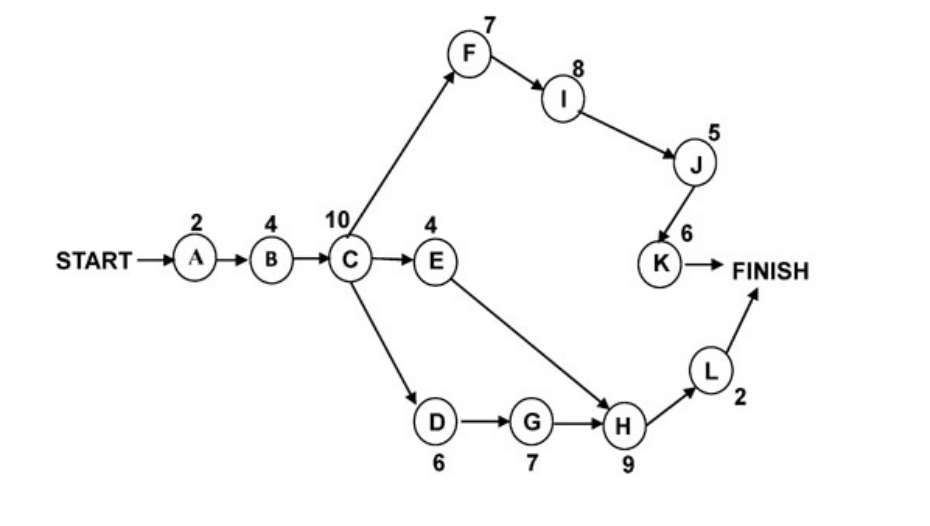
\includegraphics[scale=0.5]{q23s2}
              \label{fig:q23s2}
          \end{figure}

          The number of hours required for each activity is shown alongside the nodes. The slack on the activity $\mathbf{L}$, is \underline{\hspace{2cm}} hours.

    \item In a furnace, the inner and outer sides of the brick wall ($k_1 = 2.5~\text{W/m.K}$) are maintained at $1100^\circ$C and $700^\circ$C, respectively as shown in figure.

          \begin{figure}[H]
              \centering
              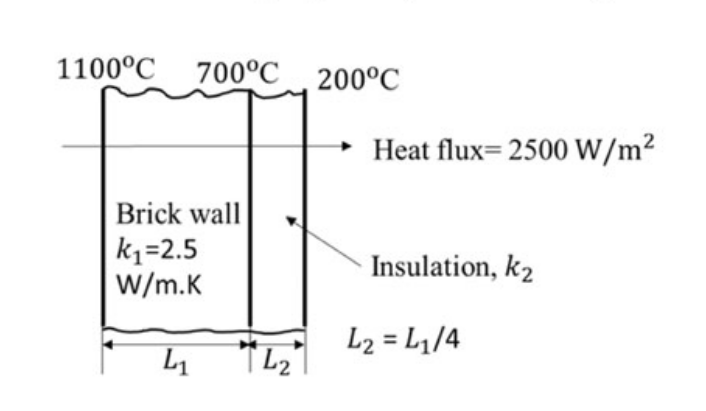
\includegraphics[scale=0.5]{q24s2}
              \label{fig:q24s2}
          \end{figure}

          The brick wall is covered by an insulating material of thermal conductivity $k_2$. The thickness of the insulation is $1/4$th of the thickness of the brick wall. The outer surface of the insulation is at $200^\circ$C. The heat flux through the composite walls is $2500~\text{W/m}^2$.

          The value of $k_2$ is \underline{\hspace{2cm}} W/m.K (\textit{round off to one decimal place}).

    \item If a reversed Carnot cycle operates between the temperature limits of $27^\circ$C and $-3^\circ$C, then the ratio of the COP of a refrigerator to that of a heat pump (COP of refrigerator / COP of heat pump) based on the cycle is \underline{\hspace{2cm}} (\textit{round off to 2 decimal places}).
\end{enumerate}

\noindent\textbf{Q26 - Q55 carry two marks each.}
\begin{enumerate}
    \setcounter{enumi}{25}
    \item The directional derivative of $f(x, y, z) = xyz$ at point $(-1, 1, 3)$ in the direction of vector $\hat{i} - 2\hat{j} + 2\hat{k}$ is
          \begin{enumerate}
              \begin{multicols}{4}
                  \item $3\hat{i} - 3\hat{j} - \hat{k}$
                  \item $-\frac{7}{3}$
                  \item $\frac{7}{3}$
                  \item $7$
              \end{multicols}
          \end{enumerate}

    \item The function $f(z)$ of complex variable $z = x + i y$, where $i = \sqrt{-1}$, is given as $f(z) = (x^3 - 3x y^2) + i\, v(x, y)$. For this function to be analytic, $v(x, y)$ should be
          \begin{enumerate}
              \begin{multicols}{2}
                  \item $(3x y^2 - y^3) + \text{constant}$
                  \item $(3x^2 y^2 - y^3) + \text{constant}$
                  \item $(x^3 - 3x^2 y) + \text{constant}$
                  \item $(3x^2 y - y^3) + \text{constant}$
              \end{multicols}
          \end{enumerate}

    \item A cantilever of length $l$, and flexural rigidity $EI$, stiffened by a spring of stiffness $k$, is loaded by a transverse force $P$, as shown.
          \begin{figure}[H]
              \centering
              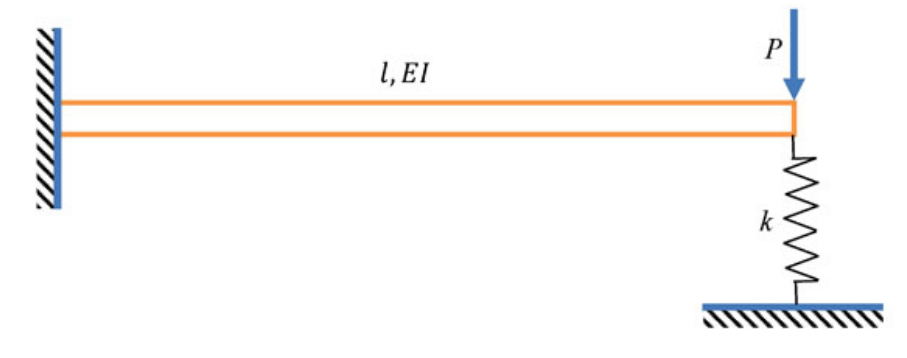
\includegraphics[scale=0.5]{q28s2}
              \label{fig:q28s2}
          \end{figure}
          The transverse deflection under the load is
          \begin{enumerate}
              \item $\dfrac{P l^3}{3EI} \left[ \dfrac{3EI}{3EI + 2k l^3} \right]$
              \item $\dfrac{P l^3}{3EI} \left[ \dfrac{6EI - k l^3}{6EI} \right]$
              \item $\dfrac{P l^3}{3EI} \left[ \dfrac{3EI - k l^3}{3EI} \right]$
              \item $\dfrac{P l^3}{3EI} \left[ \dfrac{3EI}{3EI + k l^3} \right]$
          \end{enumerate}

    \item The sun (S) and the planet (P) of an epicyclic gear train shown in the figure have identical number of teeth.


          \begin{figure}[H]
              \centering
              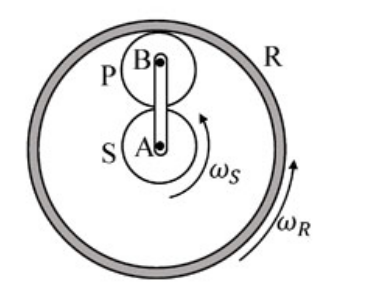
\includegraphics[scale=0.4]{q29s2}
              \label{fig:q29s2}
          \end{figure}

          If the sun (S) and the outer ring (R) gears are rotated in the same direction with angular speed $\omega_S$ and $\omega_R$, respectively, then the angular speed of the arm AB is
          \begin{enumerate}
              \item $\dfrac{3}{4}\omega_R + \dfrac{1}{4}\omega_S$
              \item $\dfrac{1}{4}\omega_R + \dfrac{3}{4}\omega_S$
              \item $\dfrac{1}{2}\omega_R - \dfrac{1}{2}\omega_S$
              \item $\dfrac{3}{4}\omega_R - \dfrac{1}{4}\omega_S$
          \end{enumerate}

    \item A thin-walled cylinder of radius $r$ and thickness $t$ is open at both ends, and fits snugly between two rigid walls under ambient conditions, as shown in the figure.

          \begin{figure}[H]
              \centering
              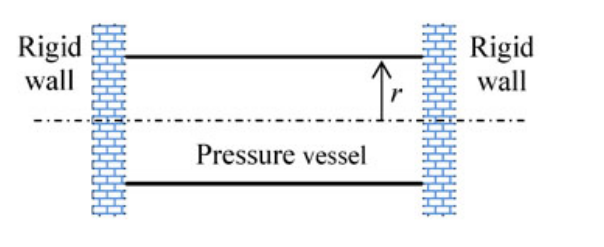
\includegraphics[scale=0.4]{q30s2}
              \label{fig:q30s2}
          \end{figure}

          The material of the cylinder has Young’s modulus $E$, Poisson’s ratio $\nu$, and coefficient of thermal expansion $\alpha$. What is the minimum rise in temperature $\Delta T$ of the cylinder (assume uniform cylinder temperature with no buckling of the cylinder) required to prevent gas leakage if the cylinder has to store the gas at an internal pressure of $p$ above the atmosphere?
          \begin{enumerate}
              \item $\Delta T = \dfrac{3 v p r}{2 \alpha t E}$
              \item $\Delta T = \left( v - \dfrac{1}{4} \right) \dfrac{p r}{\alpha t E}$
              \item $\Delta T = \dfrac{v p r}{\alpha t E}$
              \item $\Delta T = \left( v + \dfrac{1}{2} \right) \dfrac{p r}{\alpha t E}$
          \end{enumerate}
    \item A helical spring has spring constant $k$. If the wire diameter, spring diameter and the number of coils are all doubled then the spring constant of the new spring becomes
          \begin{enumerate}
              \item $k/2$
              \item $k$
              \item $8k$
              \item $16k$
          \end{enumerate}

    \item Two rollers of diameters $D_1$ (in mm) and $D_2$ (in mm) are used to measure the internal taper angle in the V-groove of a machined component. The heights $H_1$ (in mm) and $H_2$ (in mm) are measured by using a height gauge after inserting the rollers into the same V-groove as shown in the figure.

          \begin{figure}[H]
              \centering
              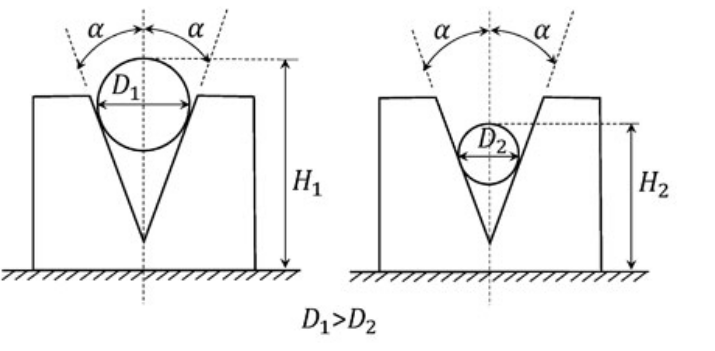
\includegraphics[scale=0.4]{q32s2}
              \label{fig:q32s2}
          \end{figure}

          Which one of the following is the correct relationship to evaluate the angle $\alpha$ as shown in the figure?
          \begin{enumerate}
              \item $\sin\alpha = \dfrac{(D_1-D_2)}{2(H_1-H_2)-(D_1-D_2)}$
              \item $\cos\alpha = \dfrac{(D_1-D_2)}{2(H_1-H_2)-2(D_1-D_2)}$
              \item $\csc\alpha = \dfrac{(H_1-H_2)-(D_1-D_2)}{2(D_1-D_2)}$
              \item $\sin\alpha = \dfrac{(H_1-H_2)}{(D_1-D_2)}$
          \end{enumerate}

    \item The forecast for the monthly demand of a product is given in the table below.

          \begin{table}[H]
              \centering
              \begin{tabular}{|c|c|c|}
                  \hline
                  \textbf{Month} & \textbf{Forecast} & \textbf{Actual Sales} \\\hline
                  1              & 32.00             & 30.00                 \\\hline
                  2              & 31.80             & 32.00                 \\\hline
                  3              & 31.82             & 30.00                 \\\hline
              \end{tabular}
              \label{tab:q33}
          \end{table}

          The forecast is made by using the exponential smoothing method. The exponential smoothing coefficient used in forecasting the demand is
          \begin{enumerate}
              \begin{multicols}{4}
                  \item 0.10
                  \item 0.40
                  \item 0.50
                  \item 1.00
              \end{multicols}
          \end{enumerate}

    \item One kg of air in a closed system undergoes an irreversible process from an initial state of $p_1 = 1$ bar (absolute) and $T_1 = 27^\circ$C, to a final state of $p_2 = 3$ bar (absolute) and $T_2 = 127^\circ$C. If the gas constant of air is 287 J/kg.K and the ratio of the specific heats $\gamma = 1.4$, then the change in the specific entropy (in J/kg.K) of the air in the process is
          \begin{enumerate}
              \item $-26.3$
              \item $28.4$
              \item $172.0$
              \item indeterminate, as the process is irreversible
          \end{enumerate}

    \item For the integral $\int_0^{\pi/2} (8 + 4\cos x) dx$, the absolute percentage error in numerical evaluation with the Trapezoidal rule, using only the end points, is \underline{\hspace{2cm}} (\textit{round off to one decimal place}).

    \item A fair coin is tossed 20 times. The probability that `head' will appear exactly 4 times in the first ten tosses, and `tail' will appear exactly 4 times in the next ten tosses is \underline{\hspace{2cm}} (\textit{round off to 3 decimal places}).

    \item A hollow spherical ball of radius 20 cm floats in still water, with half of its volume submerged. Taking the density of water as 1000 kg/m$^3$, and the acceleration due to gravity as 10 m/s$^2$, the natural frequency of small oscillations of the ball, normal to the water surface is \underline{\hspace{2cm}} radians/s (\textit{round off to 2 decimal places}).

    \item Uniaxial compression test data for a solid metal bar of length 1 m is shown in the figure.
          \begin{figure}[H]
              \centering
              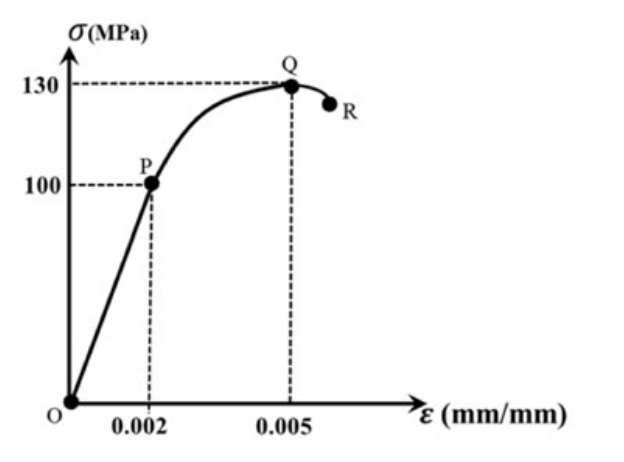
\includegraphics[scale=0.4]{q38s2}
              \label{fig:q38s2}
          \end{figure}
          The bar material has a linear elastic response from O to P followed by a nonlinear response. The point P represents the yield point of the material. The rod is pinned at both the ends. The minimum diameter of the bar so that it does not buckle under axial loading before reaching the yield point is \underline{\hspace{2cm}} mm (\textit{round off to one decimal place}).

    \item The turning moment diagram of a flywheel fitted to a fictitious engine is shown in the figure.
          \begin{figure}[H]
              \centering
              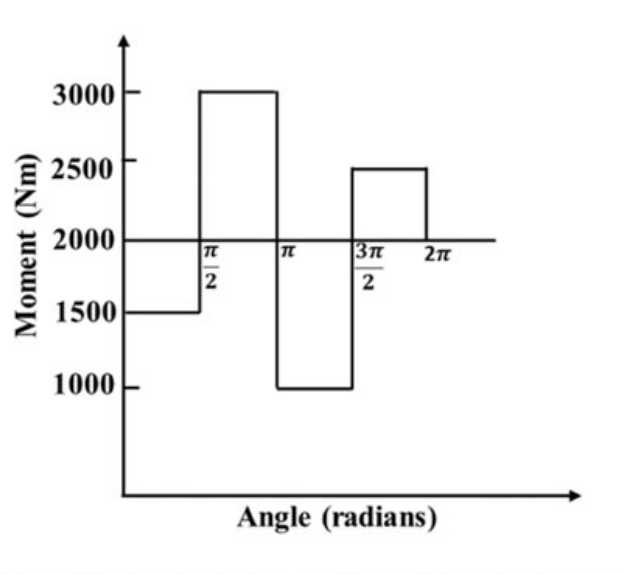
\includegraphics[scale=0.4]{q39s2}
              \label{fig:q39s2}
          \end{figure}
          The mean turning moment is 2000 Nm. The average engine speed is 1000 rpm. For fluctuation in the speed to be within $\pm2\%$ of the average speed, the mass moment of inertia of the flywheel is \underline{\hspace{2cm}} kg.m$^2$.

    \item A rigid block of mass $m_1 = 10$ kg having velocity $v_0 = 2$ m/s strikes a stationary block of mass $m_2 = 30$ kg after traveling 1 m along a frictionless horizontal surface as shown in the figure.
          \begin{figure}[H]
              \centering
              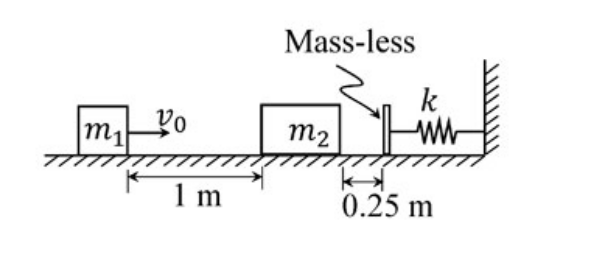
\includegraphics[width=0.5\textwidth]{q40s2}
              \label{fig:q40s2}
          \end{figure}
          The two masses stick together and jointly move by a distance of 0.25 m further along the same frictionless surface, before they touch the mass-less buffer that is connected to the rigid vertical wall by means of a linear spring having a spring constant $k = 10^5$ N/m. The maximum deflection of the spring is \underline{\hspace{2cm}} cm (\textit{round off to 2 decimal places}).

    \item A steel spur pinion has a module $(m)$ of 1.25 mm, 20 teeth and 20$^\circ$ pressure angle. The pinion rotates at 1200 rpm and transmits power to a 60 teeth gear. The face width $(F)$ is 50 mm, Lewis form factor $Y = 0.322$ and a dynamic factor $K_v = 1.26$. The bending stress $(\sigma)$ induced in a tooth can be calculated by using the Lewis formula given below.\\
          If the maximum bending stress experienced by the pinion is 400 MPa, the power transmitted is \underline{\hspace{2cm}} kW (\textit{round off to one decimal place}).\\
          Lewis formula: $\sigma = \dfrac{K_v W^t}{F m Y}$ where $W^t$ is the tangential load acting on the pinion.

    \item A mould cavity of 1200 cm$^3$ volume has to be filled through a sprue of 10 cm length feeding a horizontal runner. Cross-sectional area at the base of the sprue is 2 cm$^2$. Consider acceleration due to gravity as 9.81 m/s$^2$. Neglecting frictional losses due to molten metal flow, the time taken to fill the mould cavity is \underline{\hspace{2cm}} seconds (\textit{round off to 2 decimal places}).

    \item A cylindrical bar with 200 mm diameter is being turned with a tool having geometry $0^\circ$-$9^\circ$-$7^\circ$-$8^\circ$-$15^\circ$-$30^\circ$-$0.05$ inch (Coordinate system, ASA) resulting in a cutting force $F_{c1}$. If the tool geometry is changed to $0^\circ$-$9^\circ$-$7^\circ$-$8^\circ$-$15^\circ$-$0^\circ$-$0.05$ inch (Coordinate system, ASA) and all other parameters remain unchanged, the cutting force changes to $F_{c2}$. Specific cutting energy (in J/mm$^3$) is $U_c = U_0 (t_1)^{-0.4}$, where $U_0$ is the specific energy coefficient, and $t_1$ is the uncut thickness in mm. The value of percentage change in cutting force $F_{c2}$, i.e. $\dfrac{(F_{c2}-F_{c1})}{F_{c1}} \times 100$, is \underline{\hspace{2cm}} (\textit{round off to one decimal place}).

    \item There are two identical shaping machines S$_1$ and S$_2$. In machine S$_2$, the width of the workpiece is increased by 10\% and the feed is decreased by 10\%, with respect to that of S$_1$. If all other conditions remain the same then the ratio of total time per pass in S$_1$ and S$_2$ will be \underline{\hspace{2cm}} (\textit{round off to one decimal place}).

    \item Bars of 250 mm length and 25 mm diameter are to be turned on a lathe with a feed of 0.2 mm/rev. Each regrinding of the tool costs Rs. 20. The time required for each tool change is 1 min. Tool life equation is given as $VT^{0.2} = 24$ (where cutting speed $V$ is in m/min and tool life $T$ is in min). The optimum tool cost per piece for maximum production rate is Rs. \underline{\hspace{2cm}} (round off to 2 decimal places).

    \item A point `P' on a CNC controlled XY-stage is moved to another point `Q' using the coordinate system shown in the figure below and rapid positioning command (G00).
          \begin{figure}[H]
              \centering
              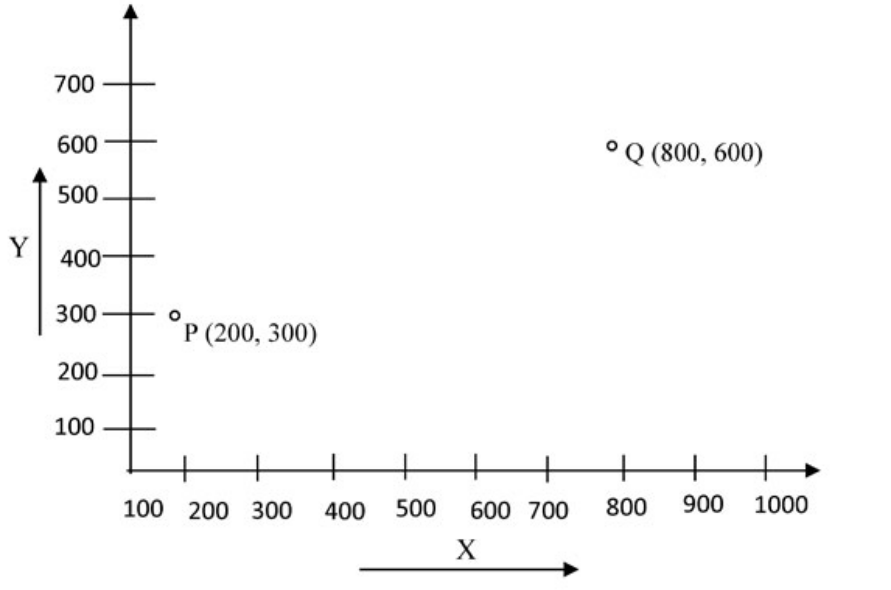
\includegraphics[width=0.9\textwidth]{q46s2}
              \label{fig:q46s2}
          \end{figure}
          A pair of stepping motors with maximum speed of 800 rpm, controlling both the X and Y motion of the stage, are directly coupled to a pair of lead screws, each with a uniform pitch of 0.5 mm. The time needed to position the point `P' to the point `Q' is \underline{\hspace{2cm}} minutes (\textit{round off to 2 decimal places}).

    \item For a single item inventory system, the demand is continuous, which is 10000 per year. The replenishment is instantaneous and backorders ($S$ units) per cycle are allowed as shown in the figure.
          \begin{figure}[H]
              \centering
              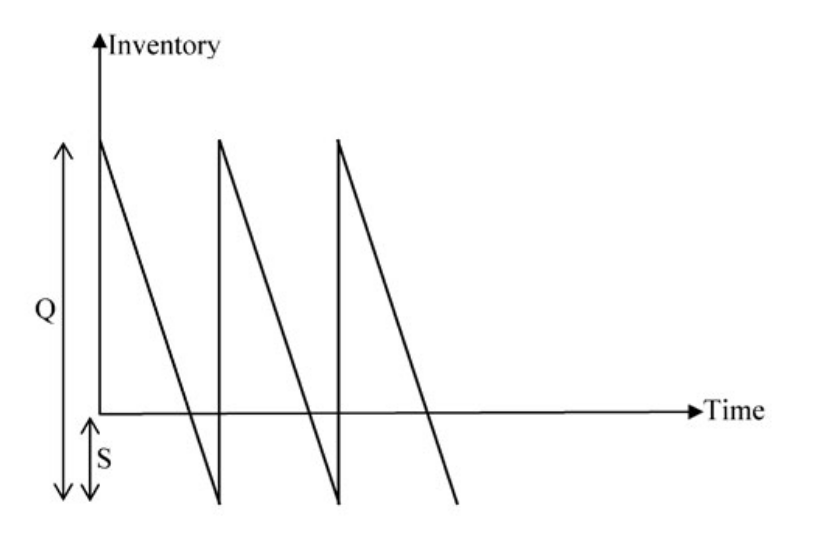
\includegraphics[width=0.9\textwidth]{q47s2}
              \label{fig:q47s2}
          \end{figure}
          As soon as the quantity ($Q$ units) ordered from the supplier is received, the backordered quantity is issued to the customers. The ordering cost is Rs. 300 per order. The carrying cost is Rs. 4 per unit per year. The cost of backordering is Rs. 25 per unit per year. Based on the total cost minimization criteria, the maximum inventory reached in the system is \underline{\hspace{2cm}} (\textit{round off to nearest integer}).

    \item Consider a flow through a nozzle, as shown in the figure below.
          \begin{figure}[H]
              \centering
              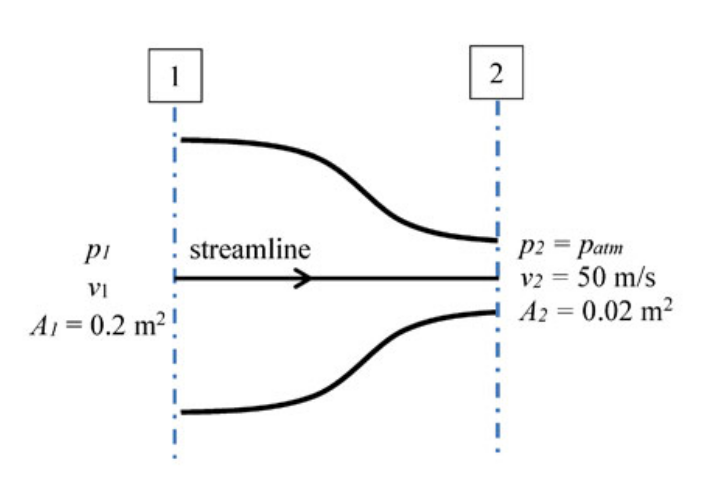
\includegraphics[width=0.5\textwidth]{q48s2}
              \label{fig:q48s2}
          \end{figure}
          The air flow is steady, incompressible and inviscid. The density of air is 1.23 kg/m$^3$. The pressure difference, $(p_1 - p_{atm})$ is \underline{\hspace{2cm}} kPa (\textit{round off to 2 decimal places}).

    \item Water (density 1000 kg/m$^3$) flows through an inclined pipe of uniform diameter. The velocity, pressure and elevation at section $\mathbf{A}$ are $V_A = 3.2$ m/s, $p_A = 186$ kPa and $z_A = 24.5$ m, respectively, and those at section $\mathbf{B}$ are $V_B = 3.2$ m/s, $p_B = 260$ kPa and $z_B = 9.1$ m, respectively. If acceleration due to gravity is 10 m/s$^2$ then the head lost due to friction is \underline{\hspace{2cm}} m (\textit{round off to one decimal place}).

    \item The spectral distribution of radiation from a black body at $T_1 = 3000$ K has a maximum at wavelength $\lambda_{max}$. The body cools down to a temperature $T_2$. If the wavelength corresponding to the maximum of the spectral distribution at $T_2$ is 1.2 times of the original wavelength $\lambda_{max}$, then the temperature $T_2$ is \underline{\hspace{2cm}} K (\textit{round off to the nearest integer}).

    \item Water flows through a tube of 3 cm internal diameter and length 20 m. The outside surface of the tube is heated electrically so that it is subjected to uniform heat flux circumferentially and axially. The mean inlet and exit temperatures of the water are 10$^\circ$C and 70$^\circ$C, respectively. The mass flow rate of the water is 720 kg/h. Disregard the thermal resistance of the tube wall. The internal heat transfer coefficient is 1697 W/m$^2\cdot$K. Take specific heat $C_p$ of water as 4.179 kJ/kg-K. The inner surface temperature at the exit section of the tube is \underline{\hspace{2cm}} $^\circ$C (\textit{round off to one decimal place}).

    \item Air is contained in a frictionless piston-cylinder arrangement as shown in the figure.

          \begin{figure}[H]
              \centering
              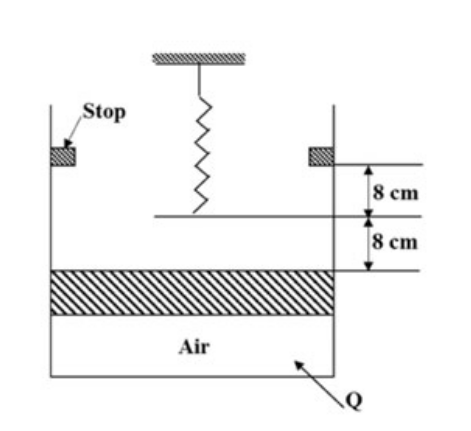
\includegraphics[width=0.5\textwidth]{q52s2}
              \label{fig:q52s2}
          \end{figure}

          The atmospheric pressure is 100 kPa and the initial pressure of air in the cylinder is 105 kPa. The area of piston is 300 cm$^2$. Heat is now added and the piston moves slowly from its initial position until it reaches the stops. The spring constant of the linear spring is 12.5 N/mm. Considering the air inside the cylinder as the system, the work interaction is \underline{\hspace{2cm}} J (\textit{round off to the nearest integer}).

    \item Moist air at 105 kPa, 30$^\circ$C and 80\% relative humidity flows over a cooling coil in an insulated air-conditioning duct. Saturated air exits the duct at 100 kPa and 15$^\circ$C. The saturation pressures of water at 30$^\circ$C and 15$^\circ$C are 4.24 kPa and 1.7 kPa respectively. Molecular weight of water is 18 g/mol and that of air is 28.94 g/mol. The mass of water condensing out from the duct is is \underline{\hspace{2cm}} g/kg of dry air (\textit{round off to 2 decimal places}).

    \item In a steam power plant, superheated steam at 10 MPa and 500$^\circ$C, is expanded isentropically in a turbine until it becomes a saturated vapour. It is then reheated at constant pressure to 500$^\circ$C. The steam is next expanded isentropically in another turbine until it reaches the condenser pressure of 20 kPa. Relevant properties of steam are given in the following two tables. The work done by both the turbines together is \underline{\hspace{2cm}} kJ/kg (\textit{round off to the nearest integer}).

          \begin{table}[H]
              \centering
              \begin{tabular}{|c|c|c|c|}
                  \hline
                  Pressure, $p$ (MPa) & Temperature, $T$ ($^\circ$C) & Enthalpy, $h$ (kJ/kg) & Entropy, $s$ (kJ/kg.K) \\
                  \hline
                  10                  & 500                          & 3373.6                & 6.5965                 \\\hline
                  1                   & 500                          & 3478.4                & 7.7621                 \\\hline
              \end{tabular}
              \caption{Superheated Steam Table}
              \label{tab:q54a}
          \end{table}


          \begin{table}[H]
              \centering
              \begin{tabular}{|c|c|c|c|c|c|}
                  \hline
                  \multirow{2}{*}{Pressure, $p$} & \multirow{2}{*}{Sat.Temp. $T_{sat}$ ($^\circ$C)} & \multicolumn{2}{|c|}{Enthalpy, $h$ (kJ/kg)} & \multicolumn{2}{|c|}{Entropy, $s$ (kJ/kg.K)}                   \\
                  \cline{3-6}
                                &                                 & $h_f$                                       & $h_g$                                        & $s_f$  & $s_g$  \\\hline
                  1 MPa         & 179.91                          & 762.9                                       & 2778.1                                       & 2.1386 & 6.5965 \\\hline
                  20 kPa        & 60.06                           & 251.38                                      & 2609.7                                       & 0.8319 & 7.9085 \\\hline
              \end{tabular}
              \caption{Saturated Steam Table}
              \label{tab:q54b}
          \end{table}

    \item Keeping all other parameters identical, the Compression Ratio (CR) of an air standard diesel cycle is increased from 15 to 21. Take ratio of specific heats = 1.3 and cut-off ratio of the cycle $r_c=2$\\\\
    The difference between the new and the old efficiency values, in percentage,\\\\
    $\left(\eta_{new}\big|_{\text{CR}=21}-\eta_{old}\big|_{\text{CR}=15}\right)$ = \underline{\hspace{2cm}} \% (\textit{round off to one decimal place}).
\end{enumerate}

\vspace{1cm}
\centering\Large\textbf{END OF THE QUESTION PAPER}

\end{document}